\documentclass[a4paper,10pt]{article}
\usepackage{amssymb,amsmath ,amsthm, graphicx}
\usepackage[left=2cm,top=2cm,right=2cm,bottom=3.5cm,nohead,nofoot]{geometry}
\usepackage{enumitem}

\usepackage[utf8]{inputenc}
\usepackage{amsfonts,amsmath,amssymb,array}

%\addtolength{\voffset}{-1cm}
%\addtolength{\hoffset}{-2cm}
%\addtolength{\textwidth}{4cm}
%\addtolength{\textheight}{2cm}

\newcommand{\lp}{\left(}
\newcommand{\rp}{\right)}
\newcommand{\lrp}[1]{\lp #1 \rp}
\newcommand{\lrb}[1]{\left[ #1 \right]}
\newcommand{\ra}{\rightarrow}
\newcommand{\la}{\leftarrow}
\newcommand{\ds}{\displaystyle}

% MATH ABBREVS
\newcommand{\eps}{\varepsilon}
\newcommand{\inv}{^{-1}}
\providecommand{\gam}{\gamma}
\providecommand{\lam}{\lambda}

% OPERATORS AND KEYWORDS
\newcommand{\kron}{\ensuremath{\otimes}}
\newcommand{\eoe}[2]{ \ve_{#1} \kron \ve_{#2} }
\newcommand{\Del}{\partial}
\DeclareMathOperator{\ave}{ave}
\DeclareMathOperator{\supp}{supp}
\DeclareMathOperator{\cut}{cut}
\DeclareMathOperator{\vol}{vol}
\DeclareMathOperator{\rank}{rank}
\DeclareMathOperator{\nullity}{nullity}
% \DeclareMathOperator{\exp}{exp}
\DeclareMathOperator{\diag}{diag}
\DeclareMathOperator{\tr}{tr}
% \DeclareMathOperator{\min}{min}
% \DeclareMathOperator{\max}{max}

% VECTORS
\providecommand{\vecn}[1]{\ensuremath{\textbf{#1}}}
\providecommand{\hvv}[1]{\hat{\vecn{#1}}}

\providecommand{\va}{\vecn{a}}
\providecommand{\vb}{\vecn{b}}
\providecommand{\vc}{\vecn{c}}
\providecommand{\vd}{\vecn{d}}
\providecommand{\ve}{\vecn{e}}
\providecommand{\vf}{\vecn{f}}
\providecommand{\vg}{\vecn{g}}
\providecommand{\vh}{\vecn{h}}
\providecommand{\vp}{\vecn{p}}
\providecommand{\vq}{\vecn{q}}
\providecommand{\vr}{\vecn{r}}
\providecommand{\vs}{\vecn{s}}
\providecommand{\vu}{\vecn{u}}
\providecommand{\vv}{\vecn{v}}
\providecommand{\vw}{\vecn{w}}
\providecommand{\vx}{\vecn{x}}
\providecommand{\vy}{\vecn{y}}
\providecommand{\vz}{\vecn{z}}
\providecommand{\vlam}{\boldsymbol{\ensuremath{\lambda}}}

% MATRICES
\newcommand{\pmat}[1]{\begin{pmatrix} #1 \end{pmatrix}}
% \newcommand{\bmat}[1]{\lrb{ \begin{array}{c} #1 \end{array} }}
\newcommand{\bmat}[1]{ \begin{bmatrix} #1 \end{bmatrix} }

\newcommand{\spmat}[1]{\left(\begin{smallmatrix} #1 \end{smallmatrix}\right)}
\newcommand{\sbmat}[1]{\left[\begin{smallmatrix} #1 \end{smallmatrix}\right]}

\providecommand{\matbld}[1]{\ensuremath{\textbf{#1}}}
\providecommand{\mA}{\matbld{A}}
\providecommand{\mB}{\matbld{B}}
\providecommand{\mC}{\matbld{C}}
\providecommand{\mD}{\matbld{D}}
\providecommand{\mE}{\matbld{E}}
\providecommand{\mF}{\matbld{F}}
\providecommand{\mG}{\matbld{G}}
\providecommand{\mH}{\matbld{H}}
\providecommand{\mI}{\matbld{I}}
\providecommand{\mJ}{\matbld{J}}
\providecommand{\mL}{\matbld{L}}
\providecommand{\mM}{\matbld{M}}
\providecommand{\mN}{\matbld{N}}
\providecommand{\mP}{\matbld{P}}
\providecommand{\mQ}{\matbld{Q}}
\providecommand{\mR}{\matbld{R}}
\providecommand{\mS}{\matbld{S}}
\providecommand{\mT}{\matbld{T}}
\providecommand{\mU}{\matbld{U}}
\providecommand{\mV}{\matbld{V}}
\providecommand{\mW}{\matbld{W}}
\providecommand{\mX}{\matbld{X}}
\providecommand{\mY}{\matbld{Y}}
\providecommand{\mZ}{\matbld{Z}}

\providecommand{\mLam}{\boldsymbol{\ensuremath{\Lambda}}}

\usepackage{csquotes}

% figure paths
\graphicspath{{.}{./figures/}}

%kyle's macros

\providecommand{\vvk}[2]{\vecn{#1}^{(#2)}}
\providecommand{\hvf}{\hvv{f}}

\newtheorem{theorem}{Theorem}
\newtheorem{lemma}{Lemma}
\newtheorem{corollary}{Corollary}
\newtheorem{proposition}{Proposition}


%% MAIN TEXT
\title{Notes on walk-entropy}
\author{Kyle Kloster}


\begin{document}
\maketitle

\abstract{
Research journal on the walk-entropy problem, which started from Blair Sullivan and I considering a conjecture from Michele Benzi~\cite{benzi2014note} regarding the relationship of the walk-regularity of a graph to the diagonal of a function of the graph's adjacency matrix.

Since NCSU undergraduate Eric Whorton joined the project, we've identified a handful more specific deceptive graphs, and eventually proved the existence of infinite families of deceptive graphs.
 }

\section{Problem Description}\label{sec:problem-statement}
%%%%%%%
%%%%%%%
%%%%      SECTION HEADING
%%%%%%%
%%%%%%%

We follow the notation and terminology laid out in the ``Spiderdonuts preliminaries" document in this project's ``background-reading" subdirectory.

Let $G$ be a standard, connected graph with adjacency matrix $\mA$. A graph is \emph{walk-regular} iff the diagonals of the powers of $\mA$ are each constant, i.e. for all $k$ we have $\diag( \mA^k ) = b_k \mI$ where for each $k$, $b_k$ is a constant. Intuitively this property means that at every length of walk $k$, every node in the graph has the same number of closed walks of length $k$. This is one sense in which a graph can be ``kind of uniform", i.e. have all nodes ``look the same". (This is distinct from the property of a graph being \emph{vertex transitive}, i.e. each node has the exact same structural property as all other nodes. Vertex transitivity is a very strict notion of node regularity -- walk-regularity is not quite as strict.)


A question central to this project is the following: given a graph $G$ and a function $f(x)$ with mild assumptions, when does the condition ``$\diag( f(\mA) )$ is a constant" imply that the graph $G$ is walk-regular? (i.e. what properties of the graph, and what properties of the function are sufficient to guarantee that statement works out?)

This originates from a conjecture of Michele Benzi's, which states that ``for any $f(x)$ with power series representation $f(x) = \sum_{k=0}^{\infty} c_k x^k$ with $c_k > 0$, if $\diag( f(\mA) )$ is constant then the graph is walk regular."
We know that a statement even stronger than the converse is true: if $G$ is walk regular, then for \emph{any} function $f$ we have that $\diag(f(\mA))$ is a constant.
Some progress has been made on the forward direction: Estrada and de la Pena showed in~\cite{estrada2014maximum} that for the specific function $f(x) = \exp(x)$ we have that ``if $\diag(\exp(\mA))$ is a constant, then $G$ is walk-regular".

However, Blair and I were able to construct a counter example to Benzi's original conjecture: we present a function $f$ satisfying Benzi's positivity property and a graph (Figure~\ref{fig:counterexample-dreidel}) that is \emph{not} walk-regular, yet the diagonal $\diag(f(\mA))$ is a constant. We call such a function ``deceptive with respect to $G$". To continue the flavor of this terminology, we would say that $\exp$ is an \emph{honest} function, since $\diag(\exp(\mA))$ being constant implies $G$ is walk-regular for \emph{any} graph $G$.

\subsection{Description of this project}
This project focuses on determining: are there classes of graphs for which all positive-power-series functions are honest? Are there classes of function that are honest with respect to all graphs? Are there \emph{straight-forward} families of graphs for which we can always construct deceptive functions?

\begin{figure}[ht]
\centering
%\hspace{1em}
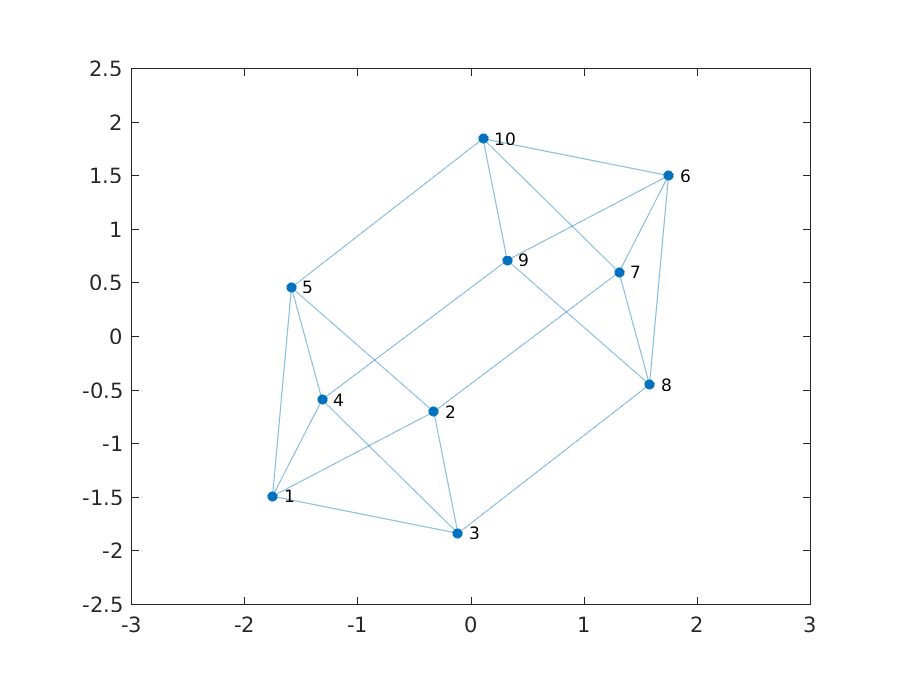
\includegraphics[width=0.7\linewidth]{walk-counterexample}%
%\hspace*{1em}
\caption{We have constructed a deceptive function for this graph, i.e. a function with constant diagonal $\diag(f(\mA))$, even though this graph is not walk-regular.}
\label{fig:counterexample-dreidel}
\end{figure}

To begin answering these questions, we first focus on some simple, individual cases. The counter-examples that Blair and I have discovered so far are all graphs with exactly two ``walk-classes" (i.e. groups of nodes with identical values in $\diag(\mA^k)$ for all $k$ ).
This setting makes it much clearer whether or not a deceptive function can be constructed.
We were able to prove that, for any non--walk-regular graph $G$ with exactly two walk-classes, a function $f$ that is deceptive with respect to $G$ can be constructed iff the two classes ``flip-flop" -- that is, if there exists one walk-length $L_1$ of which class A has more walks than class B, and a second walk-length $L_2$ of which class A has fewer walks than class B. (We make this more precise below.) For any such 2-class, non--walk-regular graph we give an explicit construction of a function that is deceptive with respect to $G$.

%We hope to generalize our counter-example construction to the case that the graph has $k$ distinct walk-classes. We have a sufficient condition (i.e. a condition on the ``flip-flopping" of the $k$ distinct node classes that is sufficient to guarantee the existence of a function that is deceptive on $G$) but we are not sure if the condition is also necessary.


\section{The two walk-class case} \label{sec:constructing-deceptive}

%%%%%%%
%%%%%%%
%%%%      SECTION HEADING
%%%%%%%
%%%%%%%

\subsection{Notation}

Let $G$ be a connected, standard graph with 2 walk-classes and that is \emph{not} walk-regular.
The goal is to construct a positive function, $f(x) = \sum_{k=0}^{\infty} c_k x^k$ with $c_k > 0 $, such that $\vf = \diag(f(\mA))$ is constant.
To proceed, we fix an arbitrary initial function, $g(x) = \sum_{k=0}^{\infty} g_k x^k$ with $g_k > 0 $ and set $\vg = \diag(g(\mA))$.
Note that, because the graph has exactly two walk-classes, the diagonal of $g(\mA)$ will have exactly two values -- one value for each node class -- and that all nodes $i$ in class $\in C_j$ will have $g(\mA)_{ii} = g_j$ a constant associated with that walk-class.

Let the classes be $C_1$ and $C_2$, and let their nodes have values in $\diag(g(\mA))$ equal to $g_1$ and $g_2$, respectively, i.e. for any nodes $i_1 \in C_1$ and $i_2 \in C_2$ we have $g(\mA)_{i_1,i_1} = g_1$ and $g(\mA)_{i_2,i_2} = g_2$.
This also holds for the diagonals of the individual powers themselves, i.e. for each class $j=1,2$ and each power $k$ we know there is some constant $\gamma(j,k)$ such that $(\mA^k)_{i_j,i_j} = \gamma(j,k)$ for all nodes $i_j$ in class $C_j$.
What this means is we can pick a single node representative for each node class, and discard the rest of the diagonal entries $(\mA^k)_{tt}$.
In a sense, this allows us to forgot about the entire graph except for two nodes, call them 1 and 2, and their diagonal values in each power $k$, $(\mA^k)_{i_j,i_j}$.

To proceed, suppose we identify a finite subset of powers (walk-lengths), $L_1, \cdots, L_t$, and look only at diagonal entries in those matrix powers, $(\mA^{L_s})_{i_j,i_j}$. (This corresponds to looking at the number of closed walks of lengths $L_1, \cdots, L_t$.)
The idea is to construct coefficients $c_k$ so that the polynomial $p(x) = \sum_{k=1} c_k x^{L_k}$ is such that we can define a \emph{new} function, $f(x) = g(x) + p(x)$ that is deceptive on $G$, i.e. $f(\mA) = g(\mA) + p(\mA)$ has constant diagonal.
To construct the appropriate coefficients $c_k$, we need to guarantee that $\vf = \diag(f(\mA))$ is constant, i.e.
\begin{align}
  \diag(g(\mA)) + \diag(p(\mA)) &= \vg + \sum_{k=1}^{t} c_k \diag(\mA^{L_k})
\end{align}
is a constant, call it $\gamma$.
By our previous logic, we really only need to check this equality on two nodes: one node representing class $C_1$ and the other respresenting class $C_2$.
In other words, we need coefficients $c_k$ and a constant $\gamma$ so that
\begin{align}
  g_1 + c_1 (\mA^{L_1})_{i_1,i_1} + \cdots + c_t (\mA^{L_t})_{i_1,i_1} &= \gamma \\
  g_2 + c_1 (\mA^{L_1})_{i_2,i_2} + \cdots + c_t (\mA^{L_t})_{i_2,i_2} &= \gamma .
\end{align}
We want to turn this into a matrix equation to solve for $c_k$. Let $\vc = [ c_1, \cdots, c_t]^T$, and create a matrix $\mM$ with $M_{j,k} = (\mA^{L_k})_{i_j,i_j}$. Finally, set $\tilde{\vg} = [ g_1, g_2 ]^T$.%, and insert the column $\mM(:,s+1) = -\ve$, where $\ve$ is the vector of all 1s of appropriate length.
Then the above system of equations can be represented by
\begin{equation}\label{eqn:class-walk-matrix1}
  \mM\vc = \gamma \ve - \tilde{\vg}.
\end{equation}
 The matrix $\mM$ is $2 \times t$, where $t$ is the number of coefficients $c_k$, which is the same as the number of different walk lengths $L_k$ (or terms $\mA^{L_k}$) that we are altering the coefficients of in $g(x)$ so that $f(\mA) = p(\mA) + g(\mA)$ has a constant diagonal.

 The question, then, is what conditions do we need on $\mM$ to guarantee a solution $\vc$ exists to~\eqref{eqn:class-walk-matrix1} satisfying $\vc > 0$ ?
 To answer the linear algebra question at face value, we will later describe and use Farkas's Lemma. But in this 2-class case, we will answer more directly.


  \begin{theorem}[2-class deception]\label{thm:2class-deceptive}
 For a non--walk-regular graph $G$ with 2 walk-classes, to be able to construct a function that is deceptive on $G$ it suffices for $G$ to have at least one walk length, $L_1$, where $(\mA^{L_1})_{i_1,i_1} > (\mA^{L_1})_{i_2,i_2}$, and at least one walk length $L_2$ where $(\mA^{L_2})_{i_1,i_1} < (\mA^{L_2})_{i_2,i_2}$. Furthermore, this condition is necessary.
  \end{theorem}

 To prove that the condition is necessary, note that if one node class, say $i_1$, is greater at every length, i.e. $(\mA^{k})_{i_1,i_1} > (\mA^{k})_{i_2,i_2}$, then no function can be constructed to be deceptive  on $G$ because for any set of positive coefficients $c_k$ we'd have $\sum_{k=0}^{\infty} c_k (\mA^{k})_{i_1,i_1} >  \sum_{k=0}^{\infty} c_k (\mA^{k})_{i_2,i_2}$. Thus, $g(\mA)_{i_1,i_1} > g(\mA)_{i_2,i_2}$, so $g$ does not have constant diagonal on $\mA$.

 We have been referring to this behavior of different node classes having the most walks of different lengths as ``flip-flopping". In the 2-class case, ``flip-flopping" happens to correspond to the matrix $\mM$ being \emph{diagonally-dominant} (i.e. in each column, the diagonal entry is larger than the sum of the absolute values of all other entries, $|M_{ii}| > \sum_{j\neq i} |M_{ji}|$). Diagonal dominance guarantees invertibility, meaning flip-flopping in the 2-by-2 case guarantees that \eqref{eqn:class-walk-matrix1} has a unique solution $\vc$. To prove that the solution is also positive, we will inspect the matrix entries. (Aside: diagonal dominance is one potential property we are considering to impose on $\mM$ in the general case to ensure the existence of deceptive functions.)

 \subsection{The construction}

 To construct an explicit deceptive function we will solve Equation~\eqref{eqn:class-walk-matrix1} by assuming, per Theorem~\ref{thm:2class-deceptive}, that the underlying graph has at least one walk-length $L_1$ for which nodes of class 1 have more walks, $(\mA^{L_1})_{i_1,i_1} > (\mA^{L_1})_{i_2,i_2}$, and at least one walk-length $L_2$ for which the reverse is true, $(\mA^{L_2})_{i_1,i_1} < (\mA^{L_2})_{i_2,i_2}$.
 Set $m_{j,k} = (\mA^{L_k})_{i_j,i_j}$ for $j=1,2$ and $k=1,2$. The choice of function $g(x)$ does not matter here, but for the sake of concreteness we will use $g(x) = \exp(x)$, and denote $g_1 = \exp(\mA)_{i_1,i_1}$ and $g_2 = \exp(\mA)_{i_2,i_2}$. Then we solve $\mM \vc = \tilde{\vg}$ by inverting $\mM = \bmat{m_{11} & m_{12} \\ m_{21} & m_{22} }$ via the standard formula:
 \[
 \vc = \tfrac{1}{m_{11}m_{22} - m_{12}m_{21}} \bmat{m_{22} & -m_{12} \\ -m_{21} & m_{11}} \bmat{\gamma - g_1 \\ \gamma - g_2}.
 \]

 Multiplication and slight algebraic rearranging yields the following:
 \begin{align}
   c_1 &= \gamma(m_{22} - m_{12}) - (m_{22}g_1 - m_{12} g_2 ) \label{eqn:defin2class-solution} \\
   c_2 &= \gamma( m_{11} - m_{21} ) - (m_{11}g_2 - m_{21}g_1)
 \end{align}

This enables us to construct a \emph{positive} solution $\vc > 0$ for any input function $g(x)$ simply by choosing $\gamma$ large enough that both $c_1$ and $c_2$ are positive, as defined in Equations~\eqref{eqn:defin2class-solution}.
We know this is possible because $m_{22}  > m_{12}$ is implied by the flip-flopping assumption we made, and so $(m_{22} - m_{12})$ is positive.
Thus, regardless of the values of $g_j$, we can always choose $\gamma$ large enough that $\gamma(m_{22} - m_{12}) > (m_{22}g_1 - m_{12} g_2 )$, and hence $c_1 > 0$.
Going through similar motions proves that $\gamma$ can be chosen large enough so that $c_2 > 0$ as well.
(This again uses the assumption we made about the diagonal entries of $\mM$ being the largest entries in their columns.)

Note that this strategy for producing a solution in fact produces an infinite number of solutions: a distinct solution is obtained by any value
\[
\gamma > \max\left\{  \frac{(m_{22}g_1 - m_{12} g_2 )}{(m_{22} - m_{12})} ~,~   \frac{(m_{11}g_2 - m_{21}g_1)}{( m_{11} - m_{21} )}  \right\}
\]
as all such values of $\gamma$ guarantee positive values for $c_1, c_2$.
Moreover, we made no assumption about the initial function $g(x)$ (other than that it is a positive-power-series function), so this strategy for producing a solution (a function that is deceptive on $G$) in fact yields an infinite family of functions that are deceptive on $G$.% even if we put limits on $\gamma$.

This completes the construction of a family of deceptive functions for a 2-class graph, assuming that the graph's two classes flip-flop.


\section{Generalizing to multiple walk-classes}


Returning to the case in which there are $k$ distinct node-walk-classes, we again want to identify conditions that will guarantee a positive solution to Equation~\eqref{eqn:class-walk-matrix1}.
The problem now is that the matrix $\mM$ is no longer $2\times 2$, so guaranteeing (1) invertibility of $\mM$ (or simply that the equation $\mM\vc = \tilde{\vg}$ is consistent), and (2) positivity of the solution, are both much more difficult, even in the $3\times 3$ case.

We have \emph{a} necessary condition for the existence of $\vc$ -- a condition we dscribed above, which we will call ``Pair-wise Flip-flop". Here are some other ideas.

\paragraph{Approaches being considered}
This is just a summary. It's unclear so far exactly which of these conditions is sufficient or necessary for Deception, and which are sufficient/necessary for Diagonal Dominance (but definitely they are all related).
\begin{enumerate}
  \item Pair-wise Flip-flop (PWFF) -- For every pair of node classes $C_i$ and $C_j$, there exists walk lengths $L_i$ and $L_j$ such that $C_i$ has more closed $L_i$-walks than $C_j$ and vice versa.
  \item All-subset Flip-flop (ASFF) -- For each subset $S$ of node-classes, there exists a walk length $L$ for which the total number of $L$-walks in $S$ is greater than the total number of $L$-walks in $S^c$.
  \item Each-Class-Max (ECM) -- for each walk-class $j$, there exists a walk-length $L_j$ such that class $j$ has more closed $L_j$-walks than any other class, i.e. $W(j,j) > W(i,j)$ for all $i\neq j$.
  \item Average Condition Flip-flop (ACFF) -- Similar to all-subset flip-flop, except we compare the average value of the subsets.
  \item Dominant Flip-flop (DFF) -- This is equivalent to ASFF and easier to state! For each node-class $C$, there exists a walk length $L$ for which the class $C$ has more $L$-walks than all other walk-classes combined.
\end{enumerate}

\textbf{Remarks:}
\begin{itemize}
  \item Dominant FF equivalent to All-subset FF
  \item Dominant/All-subset implies Each-Class-Max.
  \item Average Condition FF implies Pair-wise.
  \item Each-Class-Max implies Pair-wise.
  \item Dominant/All-subset is equivalent to the walk-class matrix being diagonally dominant!
  \item On $2\times2$, PWFF = DFF/ASFF = ECM = ACFF .
\end{itemize}


\textbf{Average Condition flip-flop.}
We say the graph satisfies the ACFF property if for each pair of subsets $S, T \neq \varnothing$ with $S \cap T = \varnothing$
there exists a length $L$ such that the following (Average Condition) holds:
\begin{equation}\label{eqn:average-condition}
  \forall j , \quad \text{average}( W(T,L) ) \leq \text{average}( W(S,L) ).
\end{equation}

An equivalent, more efficient way of thinking about this condition is:
For any subset $S$, there must exist a length $L$ such that $\text{average}( W(S,L) ) \geq \displaystyle\max_{j \notin S} \{  W(j,L)  \}$.

In words: for every subset, there must be some walk length such that that subset's average number of walks is greater than or equal to any individual class's number of walks.

Note that for ACFF we use ``$\leq$" instead of strict inequalities -- this is because of examples like this, in which the strict ACFF does not hold, but there is still a solution:

$\mM = \bmat{ 3 & 1\\ 2 & 2 \\ 1 & 3}$.

$\vx = [1; 1]$ is a solution to $\mM\vx = \ve$, but $\mM$ does not satisfy the ACFF strictly -- it satisfies it with the soft inequality $\leq$.


\section{Errors found}

The approaches I had been taking each had small errors in logic. Namely, for any argument about \emph{necessary} conditions for the existence of a deceptive function on $G$, I now believe I wasn't providing full enough context. To make clear what the error was, first we returned to a different phrasing of the originl problem:
given a graph $G$ with adjacency matrix $\mA$ does there exist a postitive function $f(x) = \sum_{k=0}^{\infty} c_k x^k$ that is deceptive on $G$, i.e. $\diag( f(\mA) )  = $ a constant. Setting $\vf = \diag(f(\mA))$ and $\vvk{d}{k} = \diag( \mA^k )$, we are asking if there exists a sequence of positive coefficients $c_k$ such that $\vf = \sum_{k=0}^{\infty} c_k \vvk{d}{k}$.

Because of the way functions behave on matrices, for any function $g(x)$ that is defined on a matrix $\mM$, there always exists a polynomial $p(x)$ with degree bounded by $n$ (the size of the square matrix $\mM$) such that $p(\mM) = f(\mM)$. I had believed this would enable us to restrict our attention to just the first $n$ terms $\vvk{d}{k}$ for $k=1,\cdots, n$ in our search for the answer to the question ``what are necessary and sufficient conditions for there to exist a deceptive function on $G$?", but the argument that I had to complete this simplification doesn't work (or, at least, it is not complete).

So, we are back to considering the infinite case: when does there exist a sequence $c_k$ such that $\vf = \mD \vc$ is a constant vector (where here we use $\mD = [ \vvk{d}{1}, \vvk{d}{2}, \cdots ]$ i.e. a $n\times \mathbb{N}$ matrix, and $\vc = [ c_1, c_2, \cdots ]$ is an $\mathbb{N}\times 1$ vector. )

There is, apparently, an infinite-dimensional version of Farka's Lemma...


For the $k$-node-walk-class case, for now I believe we have to restrict ourselves to sufficient conditions.


\section{Sufficient conditions for deception functions}

Recalling the equations
\begin{align}
  \diag(f(\mA)) &= \sum_{k=0}^{\infty} c_k \diag(\mA^k) \\
  \vf &= [ \vvk{d}{0}, \vvk{d}{1}, \cdots ] [ c_0; c_1; \cdots ] , \label{eqn:deceptive-function-vector-def}
\end{align}
 here we try to construct a finite version.
We will attempt to construct a finite matrix $\mM$ whose columns are sums of ``equivalence classes" of the columns $\vvk{d}{k}$.
First, assume we have restricted the vectors $\vvk{d}{k}$ to simply rows corresponding to the $K$ distinct node-walk-classes of the graph.
Next we construct the equivalence classes of the columns $\vvk{d}{k}$. Because there are $K$ distinct node-walk-classes, there are exactly $K!$ different possible orderings on the integers $1:K$. For each such ordering, we create an equivalence class $C_j$ of the columns $\vvk{d}{t}$ as follows: for each $t = 0,1,\cdots$, we place column $\vvk{d}{t}$ in the equivalence class $C_{j(t)}$ corresponding to the ordering on $1:K$ that a (descending) sort on $\vvk{d}{t}$ induces. Suppose there are $T$ such equivalence classes, so that $\mM$ is $K \times T$,
with column $\mM(:,j)$ being ``somehow composed of" all columns in the equivalence class $C_j$.
If we assume that there \emph{does} exist a deceptive function, i.e. coefficients $c_k >0$ such that Equation~\eqref{eqn:deceptive-function-vector-def} holds, then we can form the columns of $\mM$ as follows: $\mM(:,j) = \sum_{t \in C_j}  c_t \vvk{d}{t}$.

This construction guarantees a few things. First, the ordering on $1:K$ that defines the equivalence class $C_j$ will also apply to the column $\mM(:,j)$. Second,


\section{State of the project 2016-09-14}

Different active threads:
\begin{enumerate}
  \item\label{item:sufficient-walk-matrix} In the $k$-class case, figure out conditions on walk-class-matrix $\mW$ that are \emph{sufficient} to imply the graph is deceptive (ideas listed above, includes ASFF and PWFF for example)
  \item In the $k$-class case, figure out graph properties that are sufficient to guarantee matrix property(s) determined in~\ref{item:sufficient-walk-matrix}.
  \item In the 2-class case, determine what \emph{graph} property(s) are sufficient/necessary for the Each-Class-Max matrix condition to hold.
\end{enumerate}




\begin{theorem}[Farkas]
  Fix $\mA \in \mathbb{R}^{m \times n}$ and $\vb \in \mathbb{R}^m$. Then exactly one of the following is true:
  \begin{enumerate}
    \item There exists $\vx \geq 0$ such that $\mA\vx = \vb$, XOR
    \item There exists $\vy \in \mathbb{R}^m$ such that $\vy^T\mA \geq 0$ and $\vy^T \vb < 0$.
  \end{enumerate}
\end{theorem}

This guarantees the existence of a \emph{nonnegative} solution, $\vx \geq 0$, which does not guarantee a \emph{positive} solution $\vc > 0$ the way we want.
But! The following lemma enables us to turn any nonnegative solution to Equation~\eqref{eqn:class-walk-matrix1} into a positive solution!

Let $WR(\vx)$ denote the vector $\vx$ restricted to just one row for each walk-class. (When we use the mapping $WR$ it should not matter which node/row is used to represent any particular walk-class.)

\begin{lemma}[The ``Farkas's Lemma" lemma ]\label{thm:farkaslemmalemma}
  Suppose $g(x)$ is a positive-power-series function. Construct the walk-class matrix $\mM$ for a graph $\mA$, so that each column of $\mM$ is $WR( \diag(\mA^k))$ for some $k$.
  Next, let $\vg$ be the vector corresponding to $WR(\diag(g(\mA)))$, i.e. restricted to the distinct walk-classes.
  Let $\vx$ be any nonnegative solution to $\mM \vx = \gamma\ve - \vg$.
  Then there exists a positive-power-series function $h(x)$ different from $g(x)$ in a finite number of terms such that
  $\mM\vc = \gamma\ve - \vh$, and $\vc > 0 $, where $\vc \equiv \vx$ except on the entries where $\vx$ was zero.
\end{lemma}

% Note that the positive solution $\vc$ enables the

\begin{proof}
  Let $\vx$ be a nonnegative solution to $\mM\vx = \gamma\ve - \vg$, and
  let $\mathcal{J}$ be the index set containing the entries of $\vx$ that are zero. Note that for each $j \in \mathcal{J}$ there exists some power $p_j$ such that $\mM(:,j) = WR(\diag(\mA^{p_j}))$. Let $\mathcal{P}$ be the set of such powers, $p_j$.

  Define a new function $h(x)$ by adding to $g(x)$ a small amount at each of the terms in $\mathcal{J}$. Formally, fix any $\tau >0$ and set $h(x) = g(x) + \sum_{j \in \mathcal{J}} \tau x^{p_j}$. Thus, if we write $h(x) = \sum_{k=0}^{\infty} h_k x^k$, then we have
  \[
  h(x) = \left(\sum_{j \notin \mathcal{J}} g_j x^{p_j}\right) + \left( \sum_{j \in \mathcal{J}} (g_j + \tau) x^{p_j}\right),
  \]
  which proves that $h$ has a power-series that differs from the power-series of $g$ in a finite number of terms.

  Next, note that $\vh = \vg + \tau \cdot \mM \ve$. This is because
  \begin{align}
    \vh &= \sum_{k=0}^{\infty} h_k WR(\diag(\mA^k)) \\
        &= \sum_{j \in \mathcal{J} } h_{p_j} WR(\diag(\mA^{p_j})) +  \sum_{k \notin \mathcal{P} } h_k WR(\diag(\mA^k)) \\
        &= \sum_{j \in \mathcal{J} } (g_{p_j} + \tau) WR(\diag(\mA^{p_j})) +  \sum_{k \notin \mathcal{P} } h_k WR(\diag(\mA^k)) \\
        &= \tau \sum_{j \in \mathcal{J} } WR(\diag(\mA^{p_j})) + \sum_{k \notin \mathcal{P} } h_k WR(\diag(\mA^k)) \\
        &= \tau \mM\ve_{\mathcal{J}} +\vg
  \end{align}
  as desired.
  Plugging this into the expression $\mM \vx = \gamma\ve - \vg$, we get $\mM \vx = \gamma\ve - (\vh - \tau \mM\ve_{\mathcal{J}})$, and rearranging yields the equation
  $\mM(\vx+\tau \ve_{\mathcal{J}}) = \gamma\ve - \vh$.
  Thus, $\vc = \vx + \tau\ve_{\mathcal{J}}$ is an entirely positive solution, since we defined $\mathcal{J}$ to be the set of indices of $\vx$ where $\vx$ was zero.

\end{proof}

This lemma allows us to use Farkas's Lemma to construct positive solutions for the purposes of our problem.


\section{Thoughts 2016-09-20}
\subsection{current questions}

Suppose there exists some set of $T$ distinct terms $\diag(\mA^k)$ such that the matrix $\mM$
formed from their reduced versions, $WR(\diag(\mA^k))$, is invertible.
Is it the case that there must then exist a set of $T$ terms from the indices $[2:n]$ that such that the resulting matrix $\mM$ is also invertible?

Fix a positive vector $\vp$. Suppose there exists an index set $\mathcal{J}$
and positive coefficients $c_j$ for $j \in \mathcal{J}$ such that $\vp = \sum_{j\in\mathcal{J}} c_j WR(\diag(\mA^j))$.
Is it the case that there must exist such a set $\mathcal{J}$ within the set $[2:N]$ (possibly with different, but still positive, coefficients $c_j'$)?

These questions are trying to get at the following: is the problem we are studying really about infinite sequences (power series coefficients),
or can it always be reduced to looking for a property in the first $n$ terms $WR(\diag(\mA^k))$ for $k = 1:n$?

\subsection{Applying Farkas}

What can we learn from the ``Farkas Lemma" Lemma?  Fix a $\gamma$. Farkas says there exists a solution $\vx \geq 0 $ such that $\mM\vx = (\gamma\ve - \vg)$ if and only if there exists no $\vy$ such that ($\vy^T\mM \geq 0$ and $\vy^T(\gamma\ve - \vg) < 0 $  ).
Is it possible to change $\gamma$ to force any such $\vy$ out of existence?
Let $\mathcal{N} = \{ \vy : \vy^T\mM \geq 0,  \|\vy\|_1 = 1 \}$, i.e. the (normalized) set of all potential vectors $\vy$ that could be ``anti-Farkas vectors".
In order to be an ``anti-Farkas" vector, any such $\vy$ must satisfy the second condition, $\vy^T(\gamma\ve - \vg) < 0 $, i.e.
\begin{equation}\label{eqn:anti-farkas-criterion}
  \gamma(\vy^T\ve) < \vy^T\vg
\end{equation}

Coming from the other direction, suppose there exists a solution $\vx \geq 0$ s.t. $\mM\vx = \gamma\ve - \vg$. Then, applying Farkas's Lemma, we know there can exist no $\vy \in \mathcal{N}$ such that Equation~\eqref{eqn:anti-farkas-criterion} holds.
For any $\vy \in \mathcal{N}$, we know $\|\vy\|_1 = 1$, and so we know $ \vy^T\ve \leq 1$. Thus, if $\gamma < \vy^T \vg$ then $\vy$ would satisfy Equation~\eqref{eqn:anti-farkas-criterion}.
Since there can be no such $\vy$, we know $\vy^T \vg \leq \gamma$ must be true, for all $\vy \in \mathcal{N}$.

\textbf{Idea for construction:}
Fix a vector $\vg$. Then set $\gamma := \displaystyle\sup_{ \vy \in \mathcal{N} } \{ \vy^T\vg \}$. Then we know $\vy^T \vg \leq \gamma$ for all $\vy \in \mathcal{N}$.


\section{Thoughts 2016-09-27}
\subsection{current questions}

Returning to a point from last week: we are trying to get at the following:

> is the problem we are studying really about infinite sequences (power series coefficients), or can it always be reduced to looking for a property in the first $n$ terms $WR(\diag(\mA^k))$ for $k = 1:n$?

(or some finite constant determined by $n$?).

\textbf{Claim:} Yes!

\begin{lemma}[Finite walks]\label{thm:finitewalks}
  Let graph $G$ have walk-vectors $\vd_j = \diag(\mA^j)$, and let $\mA$ have minimial polynomial of degree $m$. Let $\vb$ be any positive vector of appropriate dimension.
  If there exists a set of positive coefficients $x_j > 0 $ for $j = 0:m$ such that $WR(\sum_{j=0}^{m}  x_j \vd_j )=  \vb$, then there exists a positive power-series function $f(x)$ such that $WR(\diag( f(\mA))) = \vb$
\end{lemma}
\begin{proof}
By assumption we have found $\vx > 0 $ such that $\mW\vx =  \vb$. We will construct the appropriate function using the values $x_j > 0$.

Recall that the degree of the minimal polynomial of $\mA$ is $m$.
First we argue, using properties of the minimal polynomial of any $n\times n$ matrix, that for each index $k = (m+1) :\infty$ there exists a set of coefficients $\{ p_{k,j} \}_{j=0}^{m}$ such that
\[
\mA^k = \sum_{j=0}^{m} p_{k,j} \mA^j.
\]
This is important because it will enable us to collapse all terms $\mA^k$ for $k=(m+1):\infty$ into just the first $m$ terms $\{\mA^j\}_{j=0}^m$.
Before we can perform this collapsing, we first need to adjust the coefficients $p_{k,j}$ can be put into certain convergent sums. The motivation for this will become clear in a couple paragraphs.

For each $j$, construct a sequence $\{s_{j,k}\}_{k=m+1}^{\infty}$ so that $\left(\sum_{k=m+1}^{\infty} p_{k,j} s_{j,k} \right)$ converges to some positive value $c_j$. One example: $s_{j,k} := 2^{-k} |p_{k,j}^{-1}|$; if $p_{k,j} = 0$ then instead use $2^{-k}$. Note that $s_{j,k}$ is positive!

Next, for each $k$ define $c_k = \displaystyle \min_{j=0:m} s_{j,k}$. Then we have that $\left( \sum_{k=m+1}^{\infty} p_{k,j} c_k \right)$ converges, for each $j$. Using the example of the coefficients $s_{j,k}$ we defined above, we have $|p_{k,j}c_k| \leq 2^{-k}$, and so the magnitude of the sum $\sum_{k=m+1}^{\infty} p_{k,j} c_k$ is bounded above by $\sum_{k=m+1}^{\infty} 2^{-k}$.

Finally, for $j=0:m$, choose $c_j = x_j - \left( \sum_{k=m+1}^{\infty} p_{k,j} c_k \right)$. If any of these $c_j$ is negative, then choose $\{ c_k \}_{k=m+1}^{\infty}$ smaller so that the values $c_j = x_j - \left( \sum_{k=m+1}^{\infty} p_{k,j} c_k \right)$ are positive.
We know this is possible because the $c_k$ can be chosen as close to 0 as we like, and $x_j > 0$ by assumption; thus the difference $x_j - \left( \sum_{k=m+1}^{\infty} p_{k,j} c_k \right)$ can be made positive by choosing $c_k$ small enough.
Choosing smaller values for $c_k$ cannot cause the sums $\sum_{k=m+1}^{\infty} p_{k,j} c_k$ to fail to converge because smaller values of $c_k$ can only cause the sum to converge more rapidly.

The end result is that any positive soution $\vx$ to $\mW\vx = \vb$ enables us to construct
\begin{align}
  \sum_{j=0}^{m} x_j \vd_{j} &=  \vb \\
  \sum_{j=0}^{m} x_j \diag(\mA^j) &=  \vb \\
  \diag\left( \sum_{j=0}^{m} x_j \mA^j \right) &=  \vb \\
  \diag\left( \sum_{j=0}^{m} \left( c_j +  \sum_{k=m+1}^{\infty} p_{k,j} c_k \right) \mA^j \right) &=  \vb.
\end{align}
Rearranging the summations yields
\begin{align}
   \vb &=  \diag\left( \sum_{j=0}^{m} c_j \mA^j  + \sum_{j=0}^m \left( \sum_{k=m+1}^{\infty} p_{k,j} c_k \right) \mA^j \right) \\
  &= \diag\left( \sum_{j=0}^{m} c_j \mA^j  +  \left( \sum_{k=m+1}^{\infty} c_k \sum_{j=0}^m p_{k,j}  \mA^j \right)  \right) \\
  &= \diag\left( \sum_{j=0}^{m} c_j \mA^j  +  \left( \sum_{k=m+1}^{\infty} c_k \mA^k \right)  \right) \\
  &= \diag \left( \sum_{j=0}^{\infty} c_j \mA^j \right).
\end{align}
This completes a proof that we have constructed coefficients for a positive power-series function $f(x)$ so that $WR(\diag(f(\mA))) = \vb$, as desired.
\end{proof}

\paragraph{Remarks:}

It is not clear that this proof says anything about whether or not the existence of a deceptive function implies the existence of a positive solution $\vx$ to the equation $\mM\vx = \vb$.

However, the machinery used in the above proof \emph{does} demonstrate that a deceptive function guarantees \emph{some} solution must exist to the equation $\mM\vx = \ve$ -- but the $\vx$ produced might not be positive (!?).

Therefore: if $\mM\vx = \ve$ has \emph{no} solutions, then there are definitely not deceptive functions, i.e. $G$ is honest.

\begin{corollary}
  If $\mM\vx = \ve$ has no solutions (of any kind, not just positive solutions), then there are no deceptive functions for the underlying graph $G$, i.e. $G$ is honest.
\end{corollary}





\paragraph{Can we combine this with earlier results?}
Now we can combine this with the ``Farkas Lemma" Lemma!

Let $g(x)$ be any positive power-series function and set $\vg = WR(\diag(g(\mA)))$ and choose $\gamma$ so that $\gamma\ve - \vg$ is positive. By Lemma~\ref{thm:farkaslemmalemma} we know that any nonnegative solution to $\mM \vy = \gamma \ve -\vg$ can be turned into a positive solution $\vx$ to a slightly different equation $\mM\vx = \gamma - \vg'$ still with positive right-hand side.
By Lemma~\ref{thm:finitewalks} we now know that any positive solution $\vx$ to an equation of the form $\mM\vx = \vb$ with positive $\vb$ yields a positive power-series function $h(x)$ such that $WR( \diag (h(\mA)) ) = \vb$.


%I DON'T THINK THIS WORKS:
%
%Now, suppose there exists a deceptive function $H(x)$ so that $\vh = WR(\diag(H(\mA))) = \alpha \ve$. Scale the function so that $\alpha < 1$, then choose $\gamma = 1 - \alpha$.
%By Lemma~\ref{thm:farkaslemmalemma} we have that any nonnegative solution to $\mM\vy = \gamma\ve + \alpha\ve \ve = \ve$ will yield a positive solution to a slightly different equation $\mM\vx = \gamma\ve - \vh$; and by Lemma~\ref{thm:finitewalks} we know that any positive solution $\vx$ to $\mM\vx = \ve$ yields a deceptive function.

%Therefore, if there exists a deceptive function, then a nonnegative solution to $\mM\vx = \ve$ can construct a deceptive function. ?



\paragraph{Necessary condition for deceptiveness}

Recall the \emph{Average-Condition Flip-Flop}: we say that any matrix $\mM$ satisfies ACFF if for every pair of disjoint, non-empty subsets $S$ and $T$, there exists a column $j$ such that $\ave(\mM(T,j)) \leq \ave(\mM(S,j))$.
\begin{lemma}
  The Average-Condition Flip-Flop is a \emph{necessary} condition for the existence of a nonnegative solution to $\mM\vx = \ve$ (where $\mM$ is any matrix and $\ve$ is the vector of all 1s).
\end{lemma}
\begin{proof}
  Assume that $\mM$ does not satisfy ACFF. We will construct a vector $\vy$ such that $\vy^T\mM \geq 0$ but $\vy^T\ve < 0$, which would imply via Farkas's Lemma that there is no $\vx \geq 0$ such that $\mM\vx = \ve$.


Since we have assumed $\mM$ does not satisfy ACFF, there must exist disjoint, non-empty subsets $S,T$ such that for all columns $j$ we have $\ave(\mM(T,j)) \lneq \ave(\mM(S,j))$.

  Construct the vector $\vy$ as follows. Set $\vy(S) = 1/|1|$, and set $\vy(T) = -(1+\delta)/|T|$ for any $\delta > 0$.
  Then $\vy = \tfrac{1}{|S|}\ve_S - \tfrac{1+\delta}{|T|}\ve_T$, and we have
  \[
    \vy^T\ve = 1 - (1+\delta) = -\delta < 0
  \]
  as long as $\delta > 0$.

  Next we pick a specific $\delta > 0$ so that $\vy$ satisfies $\vy^T\mM \geq 0$.
  Note that by construction of $S$ and $T$, we know $\ave(\mM(T,j)) \lneq \ave(\mM(S,j))$ for all $j$.
  Thus, we know the quantity
  \begin{equation}
    \delta := \displaystyle\min_j \left(  \frac{\ave(\mM(S,j)) - \ave(\mM(T,j))}{\ave(\mM(T,j))}   \right)
  \end{equation}
  is positive, since   $\ave(\mM(S,j)) - \ave(\mM(T,j)) > 0$ follows from the fact that $\ave(\mM(T,j)) \lneq \ave(\mM(S,j))$ for all $j$.

  Finally, we will show that an arbitrary column, $j$, of the row vector $\vy^T\mM$ is nonnegative (i.e. $\vy^T\mM \geq 0$).
  Expanding $\vy = \tfrac{1}{|S|}\ve_S - \tfrac{1+\delta}{|T|}\ve_T$ and multiplying with column $j$ of $\mM$ we get
  \begin{align}
    (\vy^T\mM)_j &= \left(\tfrac{1}{|S|}\ve_S - \tfrac{1+\delta}{|T|}\ve_T\right)\mM(:,j) \\
    &= \ave(\mM(S,j)) - (1+\delta)\ave(\mM(T,j)) \\
    &= \ave(\mM(S,j)) - \ave(\mM(T,j)) - \delta \ave(\mM(T,j)).
  \end{align}
  By construction of $\delta$, we know that
  \begin{align}
    \delta \ave(\mM(T,j)) &=  \ave(\mM(T,j))  \displaystyle\min_i \left(  \frac{\ave(\mM(S,i)) - \ave(\mM(T,i))}{\ave(\mM(T,i))}   \right) \\
    &\leq \ave(\mM(T,j))  \left(  \frac{\ave(\mM(S,j)) - \ave(\mM(T,j))}{\ave(\mM(T,j))}   \right) \\
    &=  \ave(\mM(S,j)) - \ave(\mM(T,j))
  \end{align}
  which is always positive for all $j$ by our assumption that $\ave(\mM(S,j)) > \ave(\mM(T,j))$ for all $j$. Now since we have constructed $\delta$ so that
  $\delta \ave(\mM(T,j)) \leq   \ave(\mM(S,j)) - \ave(\mM(T,j))$ holds,
we can upperbound our string of equalities above:
\begin{align}
    (\vy^T\mM)_j &= \ave(\mM(S,j)) - \ave(\mM(T,j)) - \delta \ave(\mM(T,j)) \\
    & \geq \ave(\mM(S,j)) - \ave(\mM(T,j)) - ( \ave(\mM(S,j)) - \ave(\mM(T,j))  ) \\
    &= 0
\end{align}
proving that $(\vy^T\mM)_j \geq 0 $ for all $j$.

Thus, by Farkas's Lemma, no solution $\vx \geq 0 $ can exist to the equation $\mM\vx = \ve$.
This completes a proof that the Average-Condition Flip-Flop is necessary for the existence of $\vx \geq 0 $ solving $\mM\vx = \ve$.

\end{proof}


\paragraph{Current questions}
Can there exist deceptive functions that give rise to non-positive solutions $\vz$ to $\mM\vz = \ve$ ?
Is ``Existence of deceptive function" equivalent to ``Existence of a positive solution to $\mM\vx = \ve$" ?

We have proved one direction of this: positive-solution guarantees deceptive function.


\paragraph{Important point}

Eric just pointed out that Average Condition does *not* imply ECML as I had previously written.

DFF implies ECM and PWFF. But ACFF just implies PWFF. ACFF (and PWFF) are necessary for $\mM\vx = \ve$ to have solutions.



\section{Refining the Flip-Flop conditions}

The original statements of these FF conditions had some problems.
We try to correct things here and state the most up-to-date versions of the conditions, together with examples that show why each condition might be useful / sufficient / necessary. In some cases we have proof that a couple conditions are necessary.(No proofs yet that anything is sufficient.)


As mentioned during our first attempt at defining FF conditions, part of our design choice is motivated by the following matrix:
$\mM = \bmat{ 3 & 1 \\   2 & 2 \\ 1 & 3 }$.

This matrix *does* have an all positive solution, $\vx = [1;1]$, to the equation $\mM\vx = \ve$. Because of that, any Flip-Flop property that we want to be necessary for deceptiveness had better hold for this $\mM$ (or else $\mM$ is a counterexample to our property being necessary).

In particular, the Average Condition FF is satisfied in only the soft sense by this $\mM$. Thus, the Average Condition FF cannot use a strict inequality, or else this $\mM$ would serve as a counterexample to ACFF being necessary for deceptiveness.

\textbf{Conclusion}: Average Condition must be defined using soft-inequalities.

At the same time, using a soft-inequality for ACFF is a little problematic. Consider the following walk-class matrix for the pyrmiad-prism with 3 faces and 1 extra layer:
\begin{verbatim}
M2 = [ [3, 6, 24, 78, 279, 990, 3588, 13122, 48495, 180654]
       [4, 6, 37, 96, 432, 1378, 5581, 19608, 76412, 281278]
       [4, 2, 36, 66, 424, 1218, 5692, 19530, 81120, 298714] ]
\end{verbatim}
M2 is not deceptive, yet it satisfies Average Condition in the soft-sense!
However, this matrix does \emph{not} satisfy Pair-wise FF in the strict sense.
The reason we know this is not deceptive is because row 1 is always $\leq$ row 2 (entry-wise) -- this property is supposed to be ruled out by Pair-wise Flip-flopping, but I forgot about that when I switched PWFF to use soft inequalities.

\textbf{Conclusion}: ACFF uses soft inequalities, but PWFF uses strict inequalities.

ECM and DFF should be using strict inequalities, but I no longer believe those conditions will be very useful. I think our best bet is for a combination of ACFF(soft) and PWFF(strict) -- we already know they are both necessary, and what's more they are not equivalent, so they are ruling out different sets of non-deceptive matrices.


\section{An infinite family of deceptive graphs via the graph tensor product}
% sec-graph-tensor-product.tex

% An infinite family of deceptive graphs via the graph tensor product
% \Box give cartesian product, \otimes gives the tensor product

Given two graphs $G$ and $H$, there are a number of different ``products" defined that can produce a third, new graph that somehow combines the two. In this section we consider in particular the tensor product of two graphs, denoted $G \times H$ or by $G \otimes H$. We will use $G \otimes H$ because of a connection with the tensor product of the graphs' adjacency matrices $\mA_{G} \otimes \mA_{H} = \mA_{G \otimes H}$.

The graph $G \otimes H$ is defined as follows. Let $G = (V,E)$ and $H = (U,F)$ be graphs. Then $G\otimes H$ has one node for each tuple $(v,u)$ with $v \in V$ and $u \in U$ (so, $|V|\cdot|U|$ total nodes); then, nodes $(v_1, u_1)$ and $(v_2, u_2)$ are connected by an edge in $G \otimes H$ iff an edge connects $v_1, v_2$ in $G$ \emph{and} an edge connects $u_1, u_2$ in $H$.

\subsection{Constructing a deceptive function on a tensor graph}\label{sec:tensor-construction}

Suppose we have a deceptive graph $G$ and a walk-regular graph $H$. We will construct a function $f(x) = \sum_{k=0}^{\infty} c_k x^k$ with $c_k >0$ such that $f( \mA_{G \otimes H})$ has constant diagonal. Then, if we can show the graph $G \otimes H$ is connected (which it will be under certain conditions on $H$) we will have demonstrated it is deceptive.

To construct $f(\mA_{G \otimes H})$ to have constant diagonal, consider its diagonal entry $(\ve_i \otimes \ve_j)^T f( \mA_{G \otimes H}) (\ve_i \otimes \ve_j)$. Recall that $\mA_{G \otimes H} = \mA_{G} \otimes \mA_H$. Next we expand the power series definition of $f$ and show how we can choose $c_k$ so that this diagonal entry is a constant independent of $i, j$.
\begin{align}
  f(\mA_{G \otimes H})_{\textrm{diag}} &= (\ve_i \otimes \ve_j)^T f( \mA_{G \otimes H}) (\ve_i \otimes \ve_j) \\
  &= (\ve_i \otimes \ve_j)^T f( \mA_G \otimes \mA_H) (\ve_i \otimes \ve_j) \\
  &= (\ve_i \otimes \ve_j)^T \left( \sum_{k=0}^{\infty} c_k (\mA_{G} \otimes \mA_H)^k \right) (\ve_i \otimes \ve_j) \\
  &= \sum_{k=0}^{\infty} c_k (\ve_i^T(\mA_{G}^k)\ve_i) \otimes (\ve_j^T(\mA_H^k)\ve_j ) \\
  &= \sum_{k=0}^{\infty} c_k (\mA_{G}^k)_{ii} (\mA_H^k)_{jj}
\end{align}
By assumption, the graph $H$ is walk-regular, and so for a fixed $k$ we know $(\mA_H^k)_{jj}$ is a constant for all $j$. This let's us choose $c_k$ as follows.
Again by assumption we know that $G$ is deceptive, and so there exists a positive sequence $d_k > 0$ such that $\sum_{k=0}^{\infty} d_k (\mA_G^k)$ has constant diagonal.
We set
\[
c_k := \begin{cases}
d_k & \textrm{ if } (\mA_H^k)_{jj} = 0 \\
d_k/(\mA_H^k)_{jj} & \textrm{ otherwise.}
\end{cases}
\]
Note that it doesn't matter which value we choose for $j$ since the matrix $\mA_H^k$ has constant diagonal. Returning to our evaluation of $f(\mA_{G \otimes H})$ above, by plugging in our definition of $c_k$ we can simplify to get
\begin{align}
  f(\mA_{G\otimes H})_{\textrm{diag}} &= \sum_{k=0}^{\infty} d_k (\mA_{G}^k)_{ii},
\end{align}
and since $\sum{k=0}^{\infty}d_k \mA_G^k$ has constant diagonal (by construction of $d_k$), we have that $f(\mA_{G\otimes H})_{\textrm{diag}}$ is constant. This completes a proof of the following proposition.

\begin{proposition}
  Given a deceptive graph $G$ and a walk-regular graph $H$, we can construct a positive sequence $c_k > 0$ such that the function $f(x) = \sum_{k=0}^{\infty} c_k x^k$ has constant diagonal on the graph $G \otimes H$.
\end{proposition}

In order for us to conclude that $G \otimes H$ is \emph{deceptive} we have to show that $G \otimes H$ is connected. If it is connected, then by definition of deceptive, $G \otimes H$ is also deceptive.

\begin{corollary}
  Given a deceptive graph $G$ and a walk-regular graph $H$, if $G \otimes H$ is connected then it is also deceptive.
\end{corollary}

So, what conditions on $G$ and $H$ can guarantee that $G \otimes H$ is connected? Keep in mind we are assuming that $G$ is connected (because we assume it is deceptive, which requires connectivity). A theorem of Weichsel~(\cite{weichsel1962kronecker}, Theorem 1) states that any tensor graph $G_1 \otimes G_2$ is connected iff both $G_1$ and $G_2$ are connected and at least one of them contains a cycle of odd length.
Therefore, for any connected, walk-regular graph $H$ that contains an odd cycle, we have that $G\otimes H$ is deceptive. Note that the cycle graphs of odd length, $C_{(2k+1)}$, are an infinite family of such connected walk-regular odd-cycle graphs, and so $G \otimes C_{(2k+1)}$ gives a distinct deceptive graph for each $k \geq 1$.

\begin{corollary}
  There exist infinite families of deceptive graphs.
\end{corollary}


\section{Cartesian product graphs}\label{sec:cartesian-graph}

We suspect that a similar result will hold for the Cartesian product of two graphs $G,H$, denoted $G \Box H$. The definition of $G \Box H$ is very similar to that of $G \otimes H$ with one important difference.
The construction of the nodeset is the same: $G \Box H$ has nodes $(u, v)$ for every node $u$ of $G$ and node $v$ of $H$. Given two nodes in $G \Box H$,  $(u_1, v_1)$ and $(u_2, v_2)$, they are connected by an edge iff (1) $v_1 = v_2$ and edge $\{u_1, u_2\}$ exists in $G$ OR (2) $u_1 = u_2$ and edge $\{v_1,v_2\}$ exists in $H$. (In contrast, $G \otimes H$ would include the edge iff \emph{both} smaller edges existed.)

The adjacency matrix of $G \Box H$ is $\mA_{G \Box H} = \mA_G \otimes \mI + \mI + \mI \otimes \mA_H$. This structure is a bit more complicated than that of $\mA_{G \otimes H}$, so the proof that tensor product graphs can be deceptive does not hold for these Cartesian product graphs.

As a cute note, observe that, since $\exp(\mA + \mB) = \exp(\mA)\exp(\mB)$ for any matrices $\mA$ and $\mB$ that commute with each other, we have that $\exp( \mA_{G \Box H}) = \exp(\mA_G \otimes \mI ) \exp(\mI \otimes \mA_{H}) = \exp(\mA_G)\otimes \exp(\mA_H)$. The cute part is that if $\exp(\mA_G)$ and $\exp(\mA_H)$ have constant diagonal, then so does $\exp( \mA_{G \Box H})$ -- this means that if $\exp$ was deceptive on two different graphs $G$ and $H$, then $\exp$ would be deceptive on any $\Box$ product $G \Box H$, $G \Box (G \Box H)$, etc. (Estrada and de la Pena proved that $\exp$ cannot be deceptive on any graph, so this point is moot.)



Some useful lemmas for our exploration of when a Cartesian product graph is deceptive:

\begin{lemma}
  Showe lemma: let $\mX$ and $\mY$ be arbitrary square, symmetric matrices. Then for any positive integer power $p$,
  \[
  (\mX \otimes \mI + \mI \otimes \mY)^p = \sum_{t=0}^p \binom{p}{t} \mX^{p-t} \otimes \mY^t
  \]
\end{lemma}

\begin{lemma}
  Showe lemma: let $\mX$ and $\mY$ be arbitrary square matrices. Let $m$ be a positive integer, and $c_k$ be any coefficients.
  \begin{align}
  \sum_{k=0}^m c_k (\mX \otimes \mI + \mI \otimes \mY)^k &=
    \sum_{k=0}^m c_k \left(\sum_{s=0}^k \binom{k}{s} \mX^{k-s}\otimes \mY^s \right) \\
    &= \sum_{s=0}^m \left( \sum_{k=s}^m c_k \binom{k}{s} \mX^{k-s} \right)\otimes \mY^s
  \end{align}
\end{lemma}


Outline of progress:

\begin{itemize}
  \item We want to use our lemma that to prove deceptiveness it suffices to construct a polynomial $p(x) = \sum_{k=0}^m c_k x^k $  (rather than an infinite series) with positive coefficients such that $p(\mA)$ has constant-diagonal.
  \item Using our lemmas about graph Cartesian products, we have $p( \mA_{H \Box G}) = \sum_{s=0}^m \left( \sum_{k=s}^m c_k \binom{k}{s} \mA_H^{k-s} \right)\otimes \mA_G^s$.
  \item By assumption, $\mA_H$ is walk-regular, and so the diagonal $\diag(\mA_H^{k-s})$ are constant for each fixed $k,s$.
  \item Hence, the diagonal entries $(\ve_i \times \ve_j)^T p(\mA_{H\Box G})(\ve_i \times \ve_j) = \sum_{s=0}^m \left( \sum_{k=s}^m c_k \binom{k}{s} (\mA_H^{k-s})_{ii} \right)\otimes (\mA_G^s)_{jj}$ depend only on $j$, not on $i$.
  \item Set $h(k,s) := (\mA_H^{k-s})_{ii}$ and note the choice of $i$ does not matter. Then we've reduced the problem to choosing values $c_k$ such that $ \sum_{s=0}^m \left( \sum_{k=s}^m c_k \binom{k}{s} h(k,s) \right)\otimes (\mA_G^s)_{jj}$ is contsant for different $j$.
  \item Setting $\vv_s = \diag( \mA_G^s )$, we're really just looking for $c_k$ that make $\sum_{s=0}^m \left( \sum_{k=s}^m c_k \binom{k}{s} h(k,s) \right)\otimes \vv_s = \ve$.
  \item Set $\mV = [ \vv_0, \vv_1, \cdots, \vv_m ]$ and define the upper-triangular matrix $\mF$ as follows; for any $k \geq s$, define $\mF(s,k) = \binom{k}{s} h(k,s)$. Then we are looking for a positive solution $\vc$ to the equation $\mV\mF\vc = \ve$.
  \item We know that the existence of a positive solution $\vx$ to $\mV\vx = \ve$ implies that $G$ is deceptive. We \emph{think} that the converse is true, but have not proved it yet.
  \item Supposing that a positive solution $\vx$ exists to $\mV \vx = \ve$, then proving deceptiveness could be accomplished by constructing a positive solution $\vx$ to $\vx = \mF\vc$. We know that $\mF$ is invertible (because it is upper triangular), and $\mF$ is nonnegative. It is unclear if positive $\vx$ necessarily means $\vc = \mF\inv \vx$ is positive. (For general positive upper-triangular $\mF$ it is not the case, but we have additional structure.)
  \item Expanding the matrix equation $\mF\vc = \vx$ yields $c_m = x_m$ and $c_{j-1} = x_{j-1} - (\sum_{i=j}^m c_i F(j-1,i))$.
\end{itemize}



{\footnotesize
\bibliographystyle{amsplain}
\bibliography{all-bibliography}
}

\end{document}
